\documentclass{article}
\usepackage[a4paper, total={6in, 8in}]{geometry}
\usepackage{amsmath}
\usepackage{graphicx}
\bibliographystyle{IEEEtran}
\usepackage{caption}
\usepackage{subcaption}
\usepackage{comment}

\usepackage{boxedminipage}
%\usepackage{geometry}
\usepackage[colorlinks=true]{hyperref}
\title{Supplemental material for `Mitigating object prior-bias from sparse-projection
tomographic reconstructions'}
\begin{document}
\date{}
\maketitle
This supplementary material consists of details which we did not
include in the main paper for purposes of brevity. This document
consists of links to view our complete 3D reconstructions, an
alternate simpler motivation for the use of multiple eigenspaces, and an
alternate learning-based method to compute weights map. %We
%also include a comparison with a method in literature based on
%comments from a reviewer.

\tableofcontents

%--------------------
%--------------------------------Links to videos-------------------------------------------------

\section{Links to view our 3D reconstructions}
Here we present the 3D reconstruction results discussed in Sec.~6 of
the main paper. For each dataset, the links contain 2 videos: one
showing all the templates and test volumes, and the other showing the
reconstructed volumes by various methods. The videos are in
\verb+.avi+ format and display reconstructions in a slice-by-slice
manner.

\begin{itemize}

\item \textbf{Potato:} 

    3D Potato of size $150\times 150\times 100$ was reconstructed from 18 cone-beam view measurements.

  \url{https://www.dropbox.com/sh/w16j7pvud2lbrpx/AACCJLxgoAurT2vVKIdu-MwFa?dl=0}
\item \textbf{Sprouts:}
 
    3D Sprouts of size $130\times 130\times 130$ was reconstructed from 30 cone-beam view measurements.

    \url{https://www.dropbox.com/sh/y6s4h2p04tp1lgq/AADn2q43o7SYj10rmheMCDzZa?dl=0}
 \item \textbf{Okra:}

  3D Okra of size $338\times 338\times 123$ was reconstructed from 45 cone-beam view measurements.

  \url{https://www.dropbox.com/sh/vkol8aluzsnusfo/AABtu6-M1LKOsQjKIjxlSxUfa?dl=0}
\end{itemize}

%------------------------------------------------------
\section{Using multiple eigenspaces}

Here we present a schematic explaining the advantage of using multiple
eigenspaces within the proposed spatially-varying reconstruction
technique. This may be viewed as a simpler version of the somewhat
long algorithm described in the main paper.


\noindent \begin{boxedminipage}{\textwidth} 
{\bf Schematic 1}: Motivation behind our algorithm. (The plus $\oplus$ and the
minus $\ominus$ operators are placeholders; precise details available
in Section~5 of the main paper). 
%\vspace{0.2cm}

{\small
 Let \textcolor{blue}{prior $Q:=$ old regions ($O$)}\\
 Let \textcolor{blue}{test volume $\boldsymbol{x}:=$ old regions ($O$) $\oplus$ new regions ($N$)}\\
% \textbf{Steps:}     
    \begin{enumerate}
\item  Compute pilot reconstruction of $\boldsymbol{x}$. Let this be called $X$.\\ \textcolor{blue}{$X = O \oplus N \oplus Ar(O) \oplus Ar(N)$}, where \\ \textcolor{blue}{$Ar(O)$} denote the reconstruction artefacts that depend on the old regions, the imaging geometry and the reconstruction method, and\\
 \textcolor{blue}{$Ar(N)$} denote the reconstruction artefacts that depend on the new regions, imaging geometry and the reconstruction method.
\item  Note that \textcolor{blue}{$Q \ominus X = N \oplus Ar(O) \oplus Ar(N)$} gives the new regions, but along with lots of artefacts due to the imaging geometry (sparse views). To eliminate these unwanted artefacts, compute \textcolor{blue}{$Y = Q \oplus Ar(O)$} by simulating projections from $Q$ using the same imaging geometry used to scan $\boldsymbol{x}$, and then reconstructing a lower quality prior volume $Y$. 
    \item Note that \textcolor{blue}{$Y \ominus X = N \oplus Ar(N)$} contains the artefacts due to the new regions only. These are different for different reconstruction methods. To eliminate these method dependent artefacts, compute $Y$ and $X$ using different reconstruction methods. Let these be denoted by $Y^j$ and $X^j$ respectively.
    \item Compute
\vspace{-0.2cm}
           \textcolor{blue}{\begin{equation*}
            Y^1 \ominus X^1 = N \oplus Ar^1(N)
           \end{equation*}
\vspace{-0.5cm}
           \begin{equation*}
            Y^2 \ominus X^2 = N \oplus Ar^2(N)
           \end{equation*}}
\vspace{-0.4cm}
   \item  New regions are obtained by computing
\vspace{-0.2cm}
          \textcolor{blue}{\begin{equation*}
          (Y^1 \ominus X^1)\cap(Y^2 \ominus X^2)= N
          \end{equation*}}   
\vspace{-0.5cm}
    \item Finally, assign space-varying weights $\boldsymbol{W}$ based on step $5$.
    \end{enumerate}
\label{algo:newRegionDetection}
}
\end{boxedminipage}

%\clearpage
%----------------------------------------------------------
\section{Learning-based computation of weights map}

The value of $k$ (discussed in Sec.~6A of the main paper) is typically
dependent on the number of false positives the system can allow in
exchange for the detection of more true positives (regions of new
changes). It is this choice and not the particular type of dataset
that affects the selection of $k$. In our work, the chosen $k$
corresponds to the one that gives minimal tolerance to false
positives. However, in case one wishes to completely avoid the use of
this hyper-parameter, one can construct a binary weights-map using a
method described below.

\begin{enumerate}
\item For the purposes of training, treat one of the previously
  scanned images as test. Annotate the region of differences between
  the test and all of the previously scanned images based on domain
  knowledge.

\item Compute the difference between the pilot reconstruction of the
  test and its projection onto the eigenspace. Let this spatial map be
  called `error map'.

\item Train a Support Vector Machine (SVM) model (or any other
  classifier model) to classify patches of this error-map image into
  one of the two categories: new changes present, new changes absent.

\item Once the trained SVM model is obtained, apply the model and
  generate binary weights-map for new test images in the same
  longitudinal study.

\item Once the binary weights-map $\boldsymbol{W_b}$ is obtained, use
  these in the alternate minimization optimization described in Eq.~3
  of the main paper.
\end{enumerate}

We mention in passing that if we are to entirely avoid the other
parameters (viz. $\lambda_1$ and $\lambda_2$), the object-prior and the pilot
can be stitched in a simplistic way using the equation

$\boldsymbol{W_b}*(\rm{pilot}) + (1-\boldsymbol{W_b})*(\rm{object\textrm{ }prior})$.
The advantage of this method is that the computational time is
significantly reduced since the alternate minimization procedure is not
used. 

%Fig.~\ref{fig:okra_svm} shows results of this method on 2D okra dataset.

  \begin{comment}
\begin{equation}
%   \setlength{\belowdisplayskip}{0pt} \setlength{\belowdisplayshortskip}{0pt}
%\setlength{\abovedisplayskip}{-2pt} \setlength{\abovedisplayshortskip}{-2pt}
J_3(\boldsymbol{\theta},\boldsymbol{\alpha}) = \lVert\boldsymbol{\mathcal{R} x}-\boldsymbol{y}\rVert_2^2  + \lambda_1\lVert\boldsymbol{\theta}\rVert_1 +\lambda_2\lVert\boldsymbol{W_b}(\boldsymbol{x} - (\boldsymbol{\mu} + \sum_{k}\boldsymbol{V_k}\alpha_k))\rVert_2^2.
\label{Eq:main}
\end{equation}
\end{comment}
%\end{enumerate} 

\begin{figure}[]
    \begin{subfigure}[b]{0.32\linewidth}
        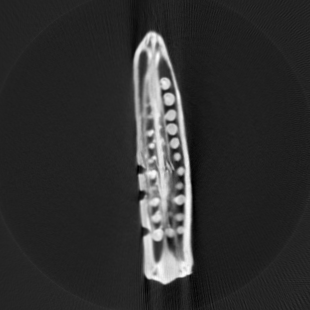
\includegraphics[width=\textwidth]{../images/svm/okra/template_1.png}
        \caption{}
     \end{subfigure}
    \begin{subfigure}[b]{0.32\linewidth}
        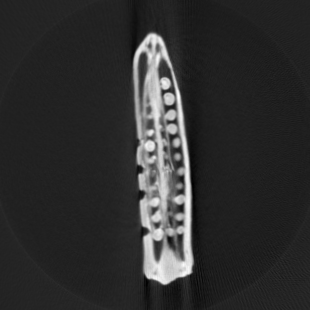
\includegraphics[width=\textwidth]{../images/svm/okra/template_2.png}
        \caption{}
     \end{subfigure}
    \begin{subfigure}[b]{0.32\linewidth}
        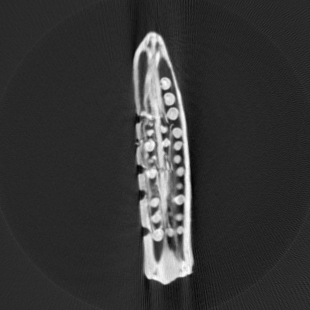
\includegraphics[width=\textwidth]{../images/svm/okra/template_3.png}
        \caption{}
     \end{subfigure}
     \begin{subfigure}[b]{0.32\linewidth}
        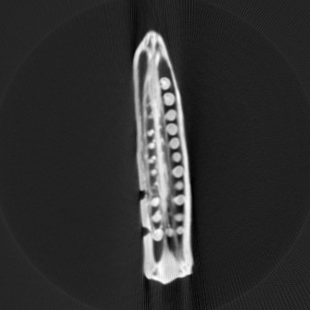
\includegraphics[width=\textwidth]{../images/svm/okra/testIm.png}
        \caption{}
     \end{subfigure}
    \begin{subfigure}[b]{0.32\linewidth}
        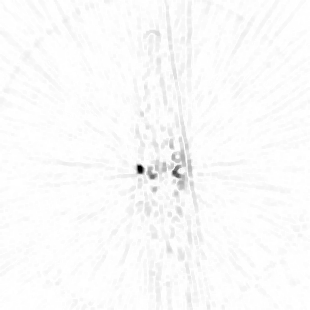
\includegraphics[width=\textwidth]{../images/svm/okra/weights.png}
        \caption{}
    \end{subfigure}
    \begin{subfigure}[b]{0.32\linewidth}
        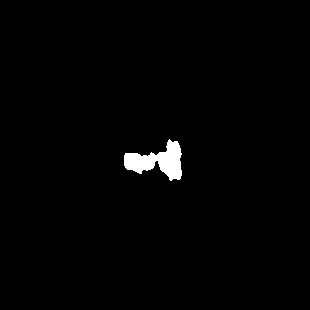
\includegraphics[width=\textwidth]{../images/svm/okra/detectedInlier.png}
        \caption{}
    \end{subfigure}
     \caption[Selecting $k$]{Using an alternate approach to generate (binary) weights map. (a)-(c) the images used as object-prior, (d) the test (310$\times$310). Measurements along $60$ views were taken. (e) error-map showing new regions, (f) detected binary weights map showing regions of new changes.}%, (g) pilot, (h) final reconstruction with pilot in the new regions, and prior in the other regions. } %(h) prior, which is obtained by projecting the pilot onto the eigenspace computed from the templates, 
\label{fig:okra_svm}
\end{figure}
%\clearpage
%\newpage





\end{document}


%----------------------------------Comparison with Literature------------------------
\section{Empirical comparison with a method in literature:\\ Detecting new changes directly in the measurements}

Sec.~2 of the main paper (`Related work') contrasts the spatially-varying technique  with other prior based techniques in literature. Here we present a 2D reconstruction  result (of the test shown in Figure.~\ref{fig:comparisonLit_dataset}) to compare our method with~\cite{Lee2012}, in which the new changes are directly detected in the measurement space by computing the difference between the measurements of the test and the corresponding simulated measurements of the template. This difference-volume is then reconstructed and then fused (added to) with the original high quality template. However, in the above method, the sub-sampling artefacts present in the difference-volume gets carried over to the final reconstructed image. This is shown in Figure~\ref{fig:comparisonLit_results}. A quantitative comparison over the region of interest is shown in Table~\ref{tab:comparisonLit}.
\begin{figure}[!h]
  \centering
    \begin{subfigure}[b]{0.24\linewidth}
        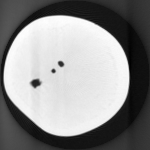
\includegraphics[width=\textwidth]{../images/potato/template_3.png}
%\captionsetup{labelformat=empty}
        \caption{Template}
     \end{subfigure}
\quad
    \begin{subfigure}[b]{0.24\linewidth}
        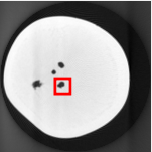
\includegraphics[width=\textwidth]{../images/potato/testIm_color.png}
%\captionsetup{labelformat=empty}
        \caption{Test}
    \end{subfigure}
    %\captionsetup{labelformat=empty}
     \caption{Template and test from the Potato dataset for the reconstructions shown in Figure.~\ref{fig:comparisonLit_results}} 
\label{fig:comparisonLit_dataset}
%\addtolength{\textfloatsep}{-0.8cm}
\end{figure}

\begin{figure}[!h]
    \begin{subfigure}[b]{0.24\linewidth}
        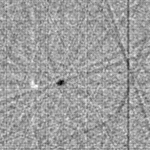
\includegraphics[width=\textwidth]{../images/comparison_lit/result_new_changes.png}
%\captionsetup{labelformat=empty}
        \caption{~\cite{Lee2012}:new-changes}
     \end{subfigure}
\quad
    \begin{subfigure}[b]{0.24\linewidth}
        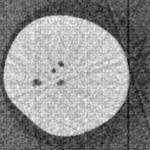
\includegraphics[width=\textwidth]{../images/comparison_lit/result_literature_test.png}
%\captionsetup{labelformat=empty}
        \caption{~\cite{Lee2012}:Reconstruction}
    \end{subfigure}
    \begin{subfigure}[b]{0.24\linewidth}
        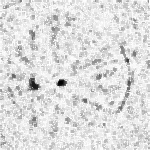
\includegraphics[width=\textwidth]{../images/comparison_lit/weightsIm_all_methods30.png}
%\captionsetup{labelformat=empty}
        \caption{Our weights-map}
    \end{subfigure}
        \begin{subfigure}[b]{0.24\linewidth}
        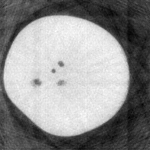
\includegraphics[width=\textwidth]{../images/comparison_lit/weighted_pca_all_methods30.png}
%\captionsetup{labelformat=empty}
        \caption{Our reconstruction}
    \end{subfigure}
    %\captionsetup{labelformat=empty}
     \caption{Reconstruction of the test in Figure~\ref{fig:comparisonLit_dataset}.  Reconstructions were performed from 12 views. Gaussian noise of 0 mean and SD = $1\%$ of mean of measurements, was added to the measurements.} 
\label{fig:comparisonLit_results}
%\addtolength{\textfloatsep}{-0.8cm}
\end{figure}

\begin{table}[!h]
  \centering
      \caption{SSIM values (within RoI) of reconstructions shown in Figure~\ref{fig:comparisonLit_results}.}
  \begin{tabular}{|l|l|l|}
\hline
 & \textbf{SSIM (whole image)} & \textbf{SSIM (RoI)} \\ \hline
\textbf{Method in~\cite{Lee2012}} & 0.65 & 0.60 \\ \hline
\textbf{\begin{tabular}[c]{@{}l@{}}This paper\end{tabular}} & 0.89 & 0.92 \\ \hline
  \end{tabular}
  \label{tab:comparisonLit}
\end{table}
%\clearpage
%\newpage
\bibliography{tci_ref}


    \begin{subfigure}[b]{0.24\linewidth}
        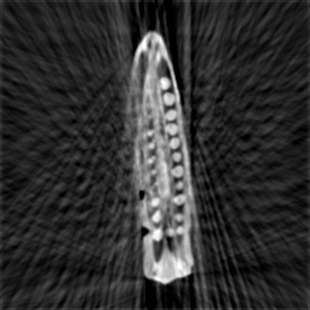
\includegraphics[width=\textwidth]{../images/svm/okra/result_pilot.png}

        \caption{}
    \end{subfigure}    
    \begin{subfigure}[b]{0.24\linewidth}
        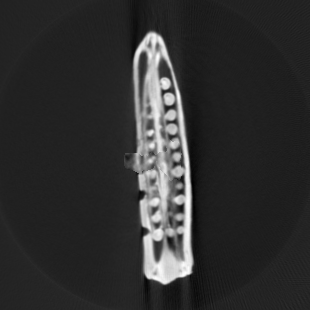
\includegraphics[width=\textwidth]{../images/svm/okra/resultStitched_svm.png}
        \caption{}
     \end{subfigure}
